% ベクトルの和：つなぐ（三角形）と平行四辺形
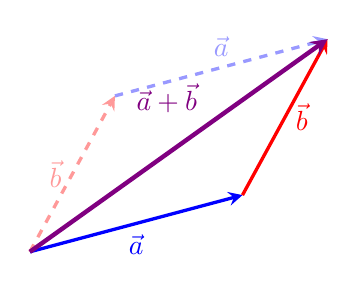
\begin{tikzpicture}[scale=0.9,>=stealth]
  \coordinate (O) at (0,0);
  \coordinate (A) at (3,0.8);
  \coordinate (C) at (4.2,3);
  \coordinate (B) at (1.2,2.2);
  \draw[->,very thick,blue] (O) -- (A) node[midway,below] {$\vec{a}$};
  \draw[->,very thick,red] (A) -- (C) node[midway,right] {$\vec{b}$};
  \draw[->,very thick,red!40,dashed] (O) -- (B) node[midway,left] {$\vec{b}$};
  \draw[->,very thick,blue!40,dashed] (B) -- (C) node[midway,above] {$\vec{a}$};
  \draw[->,ultra thick,violet] (O) -- (C) node[pos=0.6,above left] {$\vec{a}+\vec{b}$};
\end{tikzpicture}
